\documentclass[12pt, twoside]{article}
\input{../preamble}

\title{IB Math AA SL}
\author{Chris Huson}
\date{5 February 2026}

\fancyhead[LE]{\thepage}
\fancyhead[RO]{Name: \hspace{4cm} \,\\ 12th Grade \hspace{2.9cm} \,}
\fancyhead[LO]{La Scuola d'Italia / Dr.\ Huson / IB Mathematics \\* 5 February 2026}
\fancyfoot[C]{\thepage}

\begin{document}
\begin{enumerate}

\subsubsection*{Do Now: Probability exam problems}

%--- Problem 1 ---
\item In a group of 20 girls, 13 take history and 8 take economics. Three girls take both history and
economics, as shown in the following Venn diagram. The values $\boldsymbol{p}$ and $\boldsymbol{q}$
represent numbers of girls.

\begin{center}
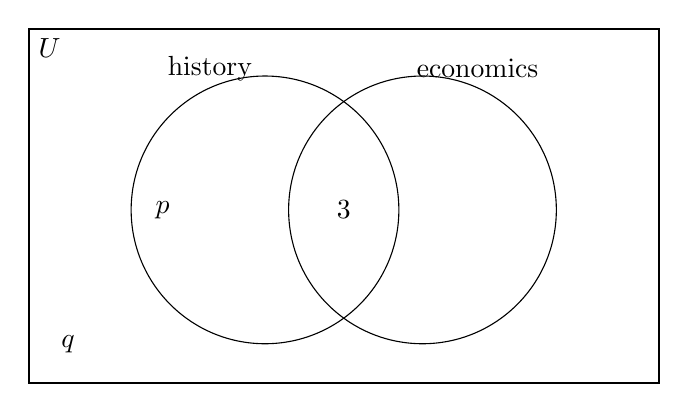
\begin{tikzpicture}
  \draw[thick] (0,0) rectangle (8,4.5);
  \node[anchor=north west] at (0,4.5) {$U$};
  \draw (3,2.2) circle (1.7cm);
  \node at (2.3,4.0) {history};
  \draw (5,2.2) circle (1.7cm);
  \node at (5.7,4.0) {economics};
  \node at (1.7,2.2) {$p$};
  \node at (4.0,2.2) {$3$};
  \node at (0.5,0.5) {$q$};
\end{tikzpicture}
\end{center}

\begin{enumerate}[itemsep=2cm]
  \item Find the value of $\boldsymbol{p}$; \hfill \textit{[2 marks]}
  \item Find the value of $\boldsymbol{q}$. \hfill \textit{[2 marks]}
  \item A girl is selected at random. Find the probability that she takes
        economics but not history. \hfill \textit{[2 marks]}
\end{enumerate}

\vspace{1cm}
\noindent\fbox{\parbox[b][6cm][t]{\dimexpr\linewidth-2\fboxsep-2\fboxrule\relax}{\textit{Working:}}}

\noindent\hfill \textbf{(Total 6 marks)}

\newpage

%--- Problem 2 ---
\item The following Venn diagram shows the events $A$ and $B$, where
$\mathrm{P}(A) = 0.4$, $\mathrm{P}(A \cup B) = 0.8$ and $\mathrm{P}(A \cap B) = 0.1$.
The values $p$ and $q$ are probabilities.

\begin{center}
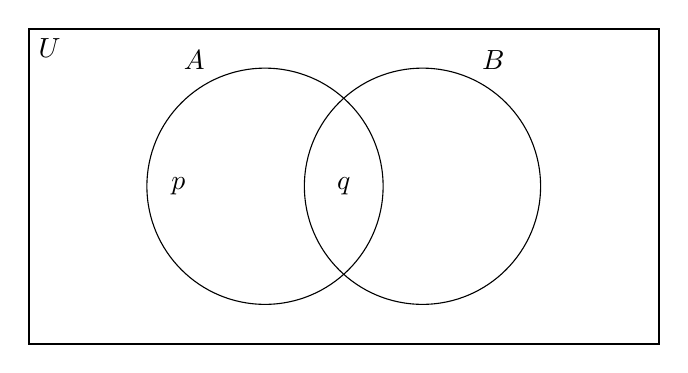
\begin{tikzpicture}
  \draw[thick] (0,0) rectangle (8,4);
  \node[anchor=north west] at (0,4) {$U$};
  \draw (3,2) circle (1.5cm);
  \node at (2.1,3.6) {$A$};
  \draw (5,2) circle (1.5cm);
  \node at (5.9,3.6) {$B$};
  \node at (1.9,2) {$p$};
  \node at (4.0,2) {$q$};
\end{tikzpicture}
\end{center}

\begin{enumerate}[itemsep=1.5cm]
  \item
    \begin{enumerate}[label=(\roman*), itemsep=0.8cm]
      \item Write down the value of $q$.
      \item Find the value of $p$. \hfill \textit{[3 marks]}
    \end{enumerate}
  \item Find $\mathrm{P}(B)$. \hfill \textit{[3 marks]}
\end{enumerate}

\vspace{1cm}

%--- Problem 3 ---
\item Events $A$ and $B$ are independent with
$\mathrm{P}(A \cap B) = 0.2$ and $\mathrm{P}(A' \cap B) = 0.6$.

\begin{enumerate}[itemsep=2cm]
  \item Find $\mathrm{P}(B)$. \hfill \textit{[2 marks]}
  \item Find $\mathrm{P}(A \cup B)$. \hfill \textit{[4 marks]}
\end{enumerate}

\vspace{1cm}

%--- Problem 4 ---
\item Nene and Deka both play netball. The probability that Nene will score a goal on her first attempt
is $0.75$. The probability that Deka will score a goal on her first attempt is $0.82$.

Calculate the probability that

\begin{enumerate}[itemsep=2cm]
  \item Nene and Deka will both score a goal on their first attempts;
  \item neither Nene nor Deka will score a goal on their first attempts. \hfill \textit{[4 marks]}
\end{enumerate}

\end{enumerate}
\end{document}
